\documentclass[letterpaper]{article}
\usepackage[utf8]{inputenc}
\usepackage[parfill]{parskip}    % Activate to begin paragraphs with an empty line rather than an indent
\usepackage{graphicx}
\usepackage{amssymb}
\usepackage{amsmath}
\usepackage{amsthm}

\usepackage{afterpage}

\usepackage{algorithm}
\usepackage{algpseudocode}

\usepackage{verse}

\newtheorem{theorem}{Theorem}[section]
\newtheorem{corollary}{Corollary}[theorem]
\newtheorem{lemma}[theorem]{Lemma}

\theoremstyle{remark}
\newtheorem*{remark}{Remark}

\usepackage{epstopdf}
\usepackage{circuitikz}
\usepackage[separate-uncertainty = true,multi-part-units=single]{siunitx}
\usepackage{booktabs}
\usepackage{enumitem}
\usepackage[toc,page]{appendix}
\usepackage{color}
\usepackage{pgfplots}
\usepackage{pgfplotstable}
\usepackage{caption}
\usepackage{subcaption}
\usepackage{url}
\usepackage{multirow}
\usepackage{makecell}
\usepackage[round]{natbib}   % omit 'round' option if you prefer square brackets
\usepackage{titling}
\usepackage{siunitx}

\usepackage{setspace}
% \doublespacing
\usepackage{float}

\pgfplotsset{compat=1.14}


\usepackage{fancyhdr}

\pgfplotscreateplotcyclelist{grayscale}{
    thick,white!10!black,mark=x,mark options=solid, dashed\\%
    thick,white!20!black,mark=o,mark options=solid\\%
}


\newcommand{\answer}[1]{\framebox{$\displaystyle #1 $}}

 
\pagestyle{fancy}
\fancyhf{}
\rhead{David Shi}
\lhead{CS61C}
\cfoot{\thepage}

\title{Lecture 3 - Notes}
\author{David Shi}
\date{June 2019}
\begin{document}

\maketitle

\section{Overview}
Last time, we covered some of the basics of C and introduced pointers. We will be diving more into the topic of pointers in this lecture, taking specifically about some specific instances of pointers such as Arrays and Strings.

\section{C Operators}

\subsection{sizeOf()}
One of the most important operators we will use is the \textbf{sizeOf()} operator. When used on a variable, the sizeOf() operator returns the number of bytes that variable or data type uses. When used on an array, sizeOf() returns the total number of bytes, calculated by taking the \textbf{Number of Indices} * \textbf{sizeOf(one element in array)}. sizeOf() a struct returns the sum of the sizeOf() all struct variables + any padding.

\subsection{Operator Precedence}
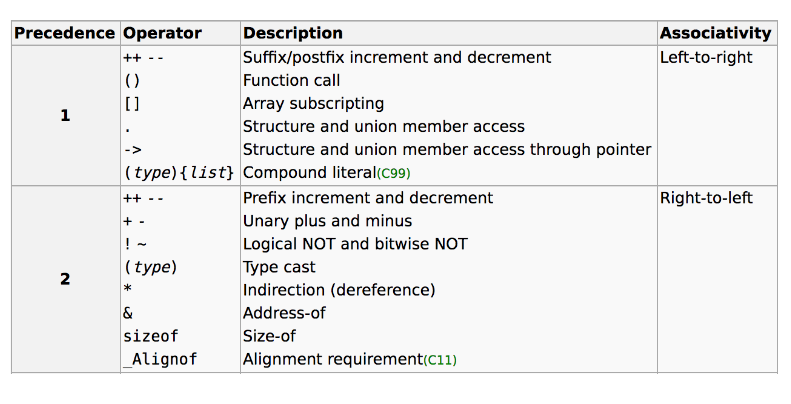
\includegraphics[scale=.5]{precedence}

The figure above explains the order of precedence operators take in C. If it is confusing, I will try to explain it further and provide examples in the following subsections.

\subsection{Assignments and Equality}
An important distinction to make that you likely already know is that \textbf{"="} is an assignment while \textbf{"=="} is testing for equality. This matches the syntax of both Java and Python. However, C is different from these two languages where assignments are allowed to take place in comparative statements. Take the following line of code for example:

\huge{if(a=b)...}

\normalsize{We can observe that this if statement does not contain an equality test \textbf{"=="} but rather an assignment statement \textbf{"="}. In Python or Java, we would be receiving an error for attempting to do this as Python and Java do not allow us to have assignments in comparative commands, such as if statements.}

Now we have to ask: how does C run an assignment within a comparative command? The answer to this is that the comparison will execute the assignment, followed by the comparison. So for the example line of code above, this if statement will be true if b is true (aka. not equal to 0 or null) and false if b is false.

Takeaway: \textbf{Assignments occur first when contained in a comparative command.}

\subsection{Precedence Note, Using Parentheses}
One helpful tip we were given is that when we are writing our own code, we should always just use parentheses to manipulate operator precedence to the \textbf{EXACT} order we want. The reason for doing this as we will see in the next few points is simply because C's Operator Precedence is really tricky and difficult to remember. It is a very strong potential pitfall for Bugs that we have no need to follow and can avoid this with a liberal use of parentheses. However, we will still study operator precedence for situations where we are given C code and we need to read it and understand what it does.

\subsection{Equality vs Logic}
If we have a line of code that has both an equality test and bitwise logic, we need to know that Equality statements bind more tightly than logic. This means that regardless of the order that the line of code is written in, the equality statement occurs first. Take the following line of code for example:

\huge{x\&1==0}

\normalsize{The way this code is written, we would likely want to interpret it as \textbf{(x\&1) == 0}}. However, because equality binds more tightly, C actually executes this code as \textbf{x\&(1==0)}. We would need parenthesis to manipulate the code to execute as the first way.

\subsection{Prefix vs Postfix}
In C, the ++ operator can be placed before or after a variable. In Java, these operators can only be placed after the variable as a postfix. When placed before, the ++ operator is a prefix (take pre to mean before), whereas placing it after is a postfix (post meaning after).

A \textbf{Prefix} takes place \textit{immediately}, whereas a \textbf{Postfix} takes place \textit{last}. Let us make int x = 1;, and observe the 2 lines of code:

int y = ++x;

int z = x++;

In the y assignment line, the ++ is placed before the variable, meaning that it is a prefix. We know that prefixes take place immediately, so x will be incremented before it is assigned to y. This means that x increments to 2, then y is assigned to 2.

In the z assignment line, the ++ is placed after the x, meaning it is a postfix. Since the post fix takes place last, z will be assigned to the value of x and then x will be incremented. So z gets assigned to x's value, which is 2. Then, x gets incremented by 1 so x becomes 3 after z is assigned.

\section{Arrays}
We will now introduce one of the most common data structures in C, and that is arrays. Arrays are a data type common to most programming languages, but there are C specific traits of arrays that we will talk about now.

\subsection{Basics}
Arrays in C are declared similarly to Java, where you can either declare it with its size specified such as 

int arr[2];

or you can initialize an array with its elements already defined, such as 

int arr = \{1, 2\}

Arrays are also zero indexed, like most other languages.

\textbf{THE BIGGEST PITFALL OF ARRAYS IN C:} arrays in C do not know their own length and do not have a function to return its length, nor does it check its bounds when being accessed. A good practice is to create a separate variable for the size of the array when it is declared/initiated. When we have an error of accessing outside of the array bounds, this is called a \textit{Segmentation Error} or \textit{Bus Error}.

\subsection{Arrays and Pointers}
It turns out that the C implementation for arrays is very similar to that of pointers. For example: int ar[] and int *ar are nearly identical in declaration. Subtle differences lie in initialization and the return value for sizeOf().

The key similarity between Arrays and Pointers that will help you understand how arrays work in C is that \textbf{an array variable acts as a pointer to its 0th element}. Because of this behavior, we can use pointer arithmetic to access across an array. We will talk about pointer arithmetic more later in this note. The two following statements are identical.

ar[0] is the same as *ar

ar[2] is the same as *(ar + 2)

Another \textbf{Important} note: Arrays in C are read-only, and we cannot reassign values inside of an array once they are initialized.


\section{Strings}
Strings in C behave as an array of characters. The two following lines of code are identical for constructing a string "abc".

char letters[] = "abc";

const char letters[] = {'a', 'b', 'c', '$\backslash$0'};

Since arrays don't know their own length, C has its last character as a '$\backslash$0' 0 byte to determine that it is the end of the string. This 0 byte is known as the \textbf{null terminator}. So to determine the length of a string, we count the number of characters until we find the null terminator. This means that there is a potential pitfall if we don't have a null terminator at the end of our string and we are at risk of a segmentation error.

\subsection{Standard C String functions}
C provides us with some handy functions for strings. Here is a quick list of a few of the most valuable basic functions:
\begin{itemize}
    \item int strlen(char *string) returns the length of the string (not including the null terminator)
    \item int strcmp(char *str1, char *str2) returns 0 if the two strings are identical in characters This differs from str1 == str2 because the '==' only checks if the two strings point to the exact same memory location
    \item char *strcpy(char *dst, char *src); copies the contents of of src to the memory location of dst. Must ensure dst has enough memory allocated to hold src. dst=src only assigns the pointer, and not the contents
\end{itemize}

\section{More on Pointers}
When we add or subtract integers from a pointer, we are moving across addresses. The amount of addresses we move depends on what kind of value the pointer points to and how much memory that value holds. For example: char *p + 1 would add 1 to the address of p because a char takes 1 byte, whereas int *p + 1 would add 4 to the address because an int takes 4 bytes. The actual operation of pointer arithmetic is the following:

p+1 = p + 1 * sizeOf(*p)

In essence, adding 1 to a pointer moves the pointer to the next value. This is useful for arrays since adding 1 to an array moves to the next value in the array.

We should be cautious of using pointer arithmetic to ensure we are getting the intended behavior, as debugging an error in pointer arithmetic will be very tedious to fix and very difficult to find.

Here is a list of valid Pointer arithmetic. Anything else is illegal as it doesn't make any practical sense:
\begin{itemize}
    \item Adding an integer to a pointer
    \item subtracting two pointers (in the same array) to find the distance between the two values in the array
    \item comparing two pointers (<, >, <=, >=, !=, ==)
    \item comparing a pointer to null
\end{itemize}

\subsection{Pointer Operator Precedence}
If more than one prefixal operator is present, they are applied from right to left. Observe the following lines of code:

*++p

--*p

The first line will increment the address of p by one to the 1st element, and then get the value in that address. The second line of code will get the value of the 0th element of p, and then subtract one from that value.

When both Prefixal and Postfixal operators are present, the prefix operator is returned, and then the postfix operator takes place afterwords. Observe the following line of code:

*p++

This statement will return the 0th element of p, and then afterwords increment p by one. This is a very useful behavior to utilize in loops.

\subsection{Pointer Allocation}
When a pointer is declared, it does not point to anything, and will point to garbage. This is a similar behavior of declaring variables without initializing them. Pointers can either point to something that already exists, or we can allocate room in memory for the new thing to point to \textit{(we will learn this next lecture)}

Pointers are also allowed to point to pointers, declared as **h. We will talk about this later as well.
\end{document}


